%%%%%%%%%%%%%%%%%%%%%%%%%%%%%%%%%%%%%%%
% Wenneker Resume/CV
% LaTeX Template
% Version 1.1 (19/6/2016)
%
% This template has been downloaded from:
% http://www.LaTeXTemplates.com
%
% Original author:
% Frits Wenneker (http://www.howtotex.com) with extensive modifications by 
% Vel (vel@LaTeXTemplates.com)
%
% License:
% CC BY-NC-SA 3.0 (http://creativecommons.org/licenses/by-nc-sa/3.0/
%
%%%%%%%%%%%%%%%%%%%%%%%%%%%%%%%%%%%%%%

%----------------------------------------------------------------------------------------
%	PACKAGES AND OTHER DOCUMENT CONFIGURATIONS
%----------------------------------------------------------------------------------------

\documentclass[a4paper,12pt]{memoir} % Font and paper size

%%%%%%%%%%%%%%%%%%%%%%%%%%%%%%%%%%%%%%%%%
% Wenneker Resume/CV
% Structure Specification File
% Version 1.1 (19/6/2016)
%
% This file has been downloaded from:
% http://www.LaTeXTemplates.com
%
% Original author:
% Frits Wenneker (http://www.howtotex.com) with extensive modifications by 
% Vel (vel@latextemplates.com)
%
% License:
% CC BY-NC-SA 3.0 (http://creativecommons.org/licenses/by-nc-sa/3.0/)
%
%%%%%%%%%%%%%%%%%%%%%%%%%%%%%%%%%%%%%%%%%

%----------------------------------------------------------------------------------------
%	PACKAGES AND OTHER DOCUMENT CONFIGURATIONS
%----------------------------------------------------------------------------------------

\usepackage{XCharter} % Use the Bitstream Charter font
\usepackage[utf8]{inputenc} % Required for inputting international characters
\usepackage[T1]{fontenc} % Output font encoding for international characters

\usepackage[top=1cm,left=1cm,right=1cm,bottom=1cm]{geometry} % Modify margins

\usepackage{graphicx} % Required for figures

\usepackage{flowfram} % Required for the multi-column layout

\usepackage{url} % URLs

\usepackage[usenames,dvipsnames]{xcolor} % Required for custom colours
\definecolor{CompanyColor}{RGB}{14,135,204}

\usepackage{tikz} % Required for the horizontal rule

\usepackage{enumitem} % Required for modifying lists
\setlist{noitemsep,nolistsep} % Remove spacing within and around lists

\setlength{\columnsep}{\baselineskip} % Set the spacing between columns

% Define the left frame (sidebar)
\newflowframe{0.25\textwidth}{\textheight}{0pt}{0pt}[left]
\newlength{\LeftMainSep}
\setlength{\LeftMainSep}{0.25\textwidth}
\addtolength{\LeftMainSep}{\columnsep}

% Small static frame for the vertical line
\newstaticframe{1.5pt}{\textheight}{\LeftMainSep}{0pt}
 
% Content of the static frame with the vertical line
\begin{staticcontents}{1}
\hfill
\tikz{\draw[loosely dotted,color=CompanyColor,line width=1.5pt,yshift=0](0,0) -- (0,\textheight);}
\hfill\mbox{}
\end{staticcontents}
 
% Define the right frame (main body)
\addtolength{\LeftMainSep}{1.5pt}
\addtolength{\LeftMainSep}{1\columnsep}
\newflowframe{0.7\textwidth}{\textheight}{\LeftMainSep}{0pt}[main01]

\pagestyle{empty} % Disable all page numbering

\setlength{\parindent}{0pt} % Stop paragraph indentation

%----------------------------------------------------------------------------------------
%	NEW COMMANDS
%----------------------------------------------------------------------------------------

\newcommand{\userinformation}[1]{\renewcommand{\userinformation}{#1}} % Define a new command for the CV user's information that goes into the left column

\newcommand{\cvheading}[1]{{\Huge\bfseries\color{CompanyColor} #1} \par\vspace{.6\baselineskip}} % New command for the CV heading
\newcommand{\cvsubheading}[1]{{\Large\bfseries #1} \bigbreak} % New command for the CV subheading

\newcommand{\Sep}{\vspace{1em}} % New command for the spacing between headings
\newcommand{\SmallSep}{\vspace{0.5em}} % New command for the spacing within headings

\newcommand{\aboutme}[2]{ % New command for the about me section
\textbf{\color{CompanyColor} #1}~~#2\par\Sep
}
	
\newcommand{\CVSection}[1]{ % New command for the headings within sections
{\Large\textbf{#1}}\par
\SmallSep % Used for spacing
}

\newcommand{\CVItem}[2]{ % New command for the item descriptions
\textbf{\color{CompanyColor} #1}\par
#2
\SmallSep % Used for spacing
}

\newcommand{\bluebullet}{\textcolor{CompanyColor}{$\circ$}~~} % New command for the blue bullets
 % Include the file specifying document layout and packages

\renewcommand{\familydefault}{\sfdefault}

\usepackage[ngerman]{babel}
\usepackage{marvosym}

\usepackage{hyperref}
\hypersetup{
	colorlinks=true,
	urlcolor=RoyalBlue,
	pdftitle={Bewerbung Moritz Schubert}
}

%----------------------------------------------------------------------------------------
%	NAME AND CONTACT INFORMATION 
%----------------------------------------------------------------------------------------

\userinformation{ % Set the content that goes into the sidebar of each page
\begin{flushright}
% Comment out this figure block if you don't want a photo
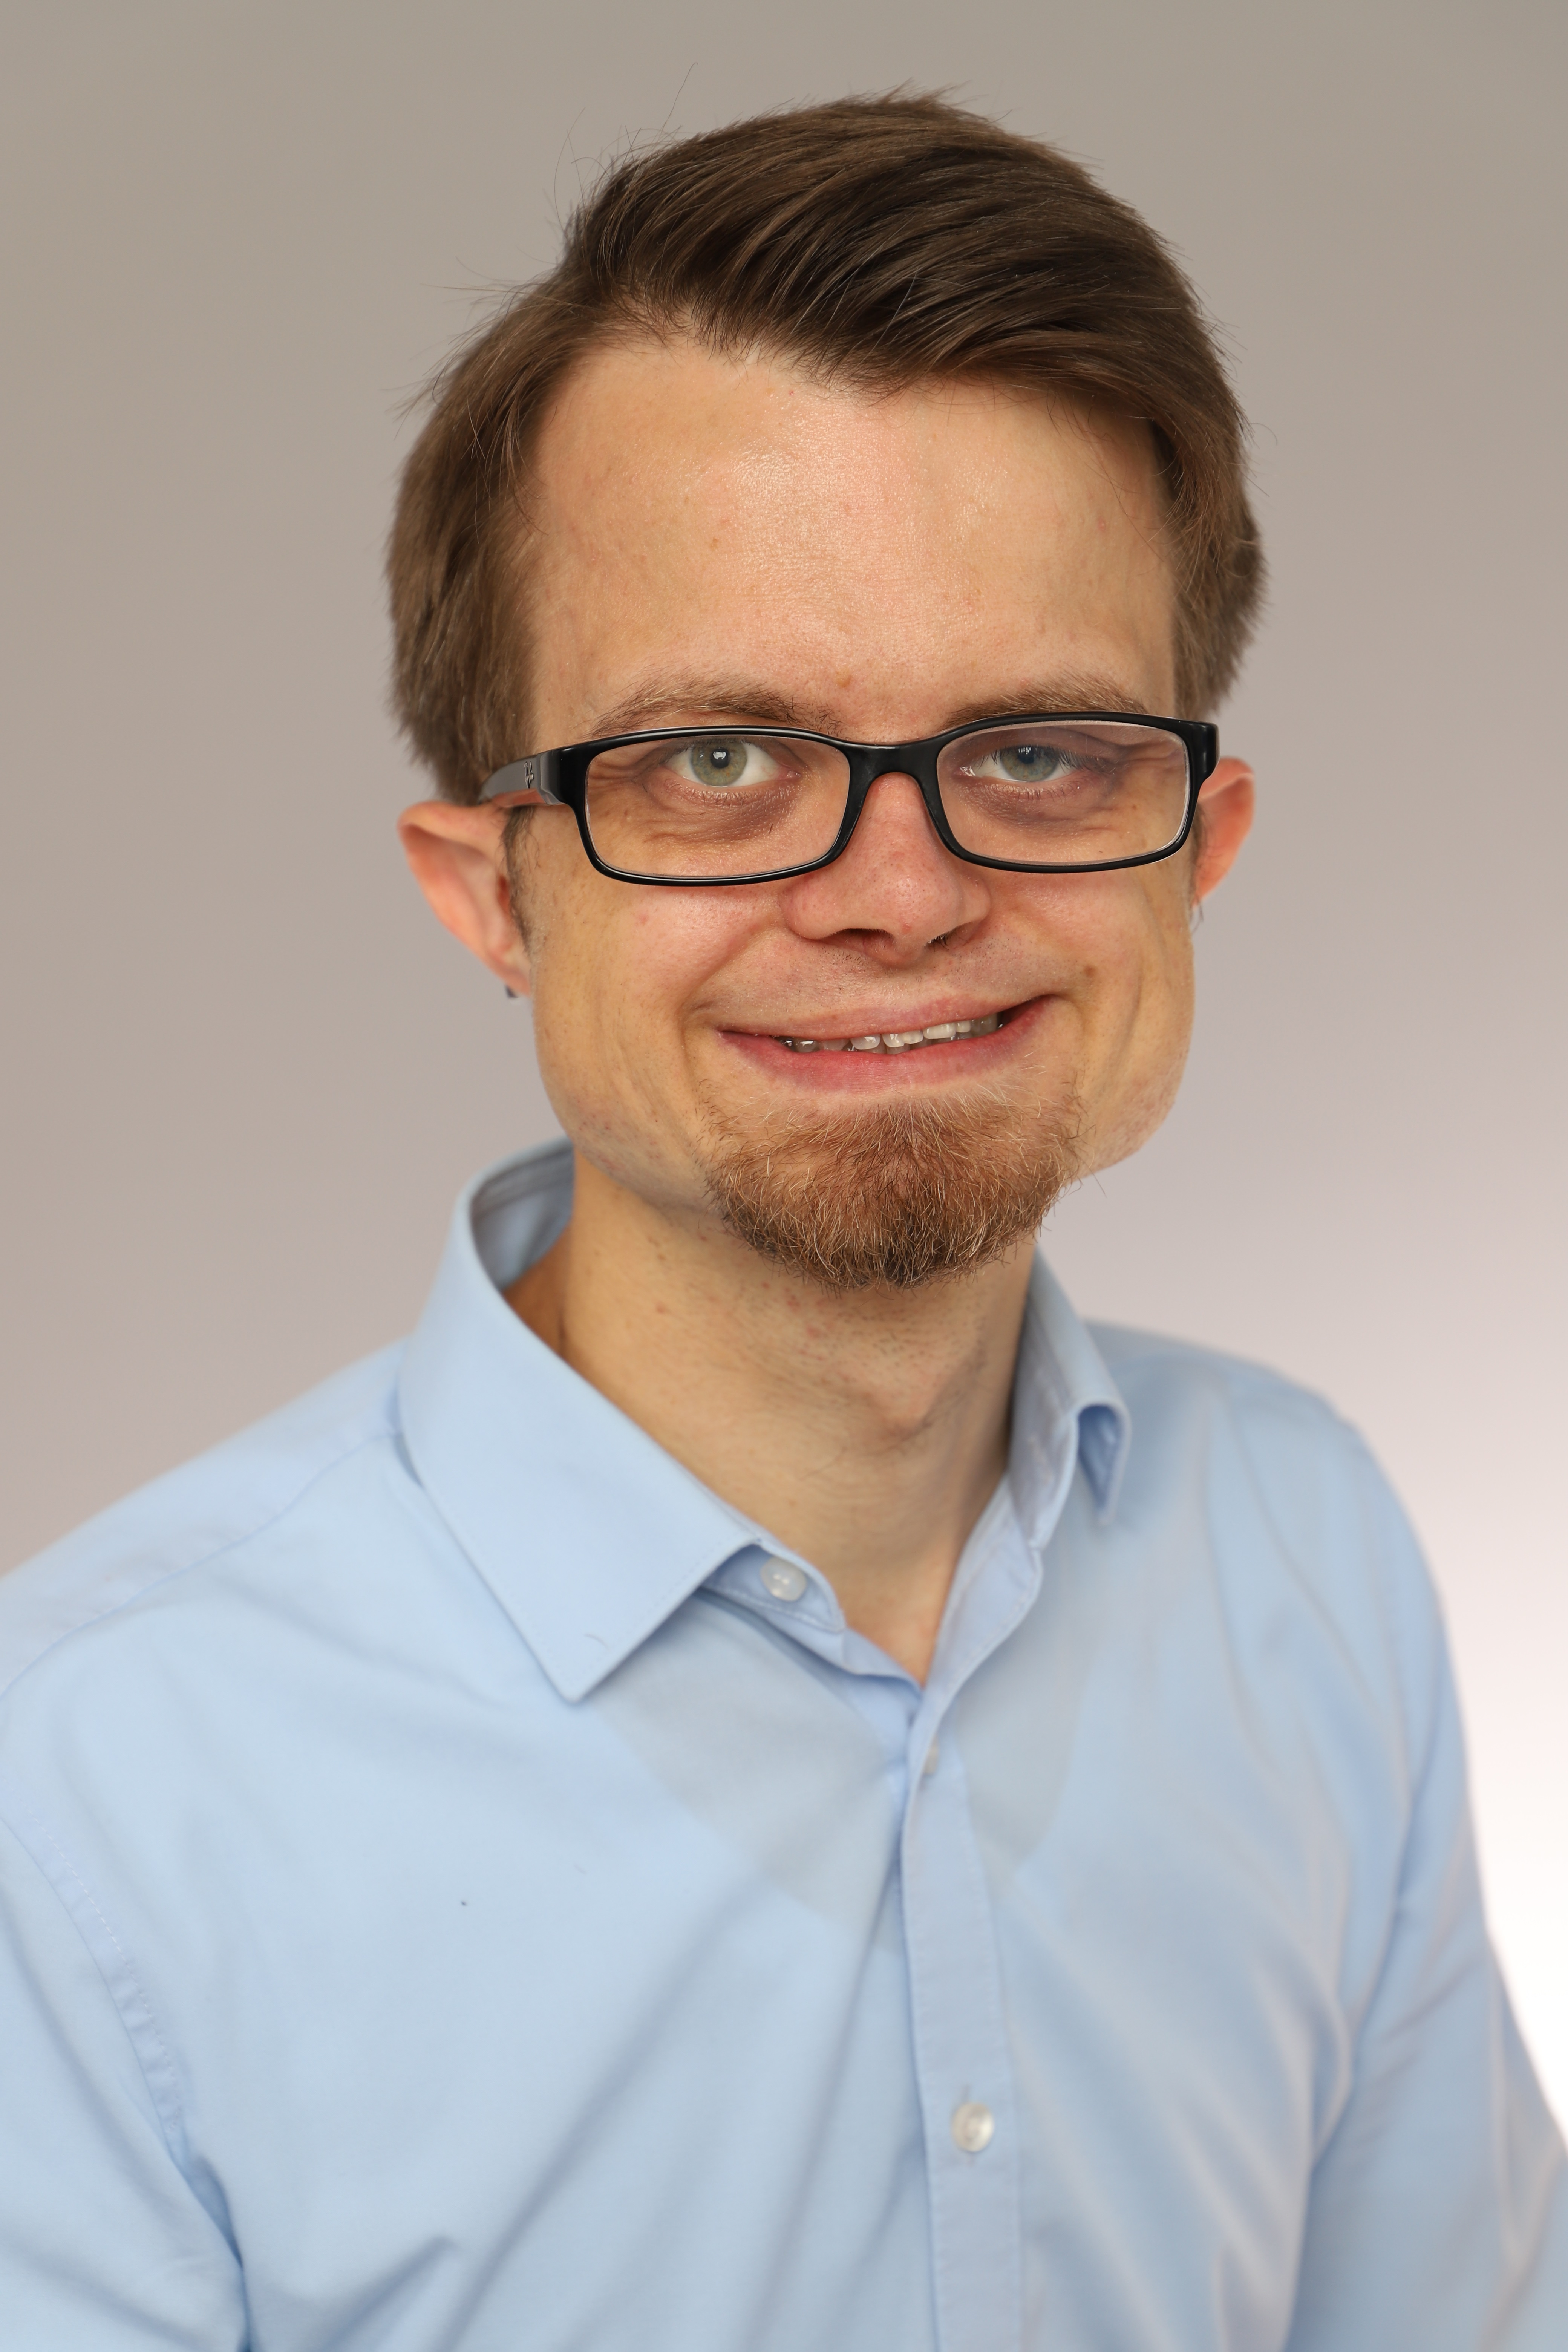
\includegraphics[width=0.6\columnwidth]{../photo.jpg}\\[\baselineskip] % Your photo
\small % Smaller font size
Marburg\\ % Address 2
\href{mailto:moritzschubert@posteo.de}{\Letter\  <vorname><nachname>\\@posteo.de}  \\ % Your email address
\Sep
\href{https://www.linkedin.com/in/moritz-schubert-data-scientist}{linkedin.com/in/moritz-schubert-data-scientist} \\ % Your URL
\Sep % Some whitespace
Nationalität: deutsch\\
Familienstand: ledig\\
\vfill % Whitespace under this block to push it up under the photo
\end{flushright}
}

%----------------------------------------------------------------------------------------

\begin{document}

\userinformation % Print your information in the left column

\framebreak % End of the first column

%----------------------------------------------------------------------------------------
%	HEADING
%----------------------------------------------------------------------------------------

\cvheading{Moritz Schubert} % Large heading - your name

\cvsubheading{Wissenschaftler} % Subheading - your occupation/specialization

\vspace{2em}

%----------------------------------------------------------------------------------------
%	EDUCATION
%----------------------------------------------------------------------------------------

\CVSection{Ausbildung}

%------------------------------------------------

\CVItem{2019--, Promotion}{Arbeitseinheit Theoretische Kognitionswissenschaften, Fachbereich Psychologie, Philipps-Universität Marburg}

%------------------------------------------------

\CVItem{2017--2019, Master Psychologie (Note 1,3)}{Philipps-Universität Marburg}

\CVItem{2012--2017, Bachelor Psychologie (Note 2,4)}{Philipps-Universität Marburg}

%------------------------------------------------

\Sep % Extra whitespace after the end of a major section

%----------------------------------------------------------------------------------------
%	EXPERIENCE
%----------------------------------------------------------------------------------------

\CVSection{Berufserfahrung}

%------------------------------------------------

\CVItem{2019--2023, \textit{wissenschaftl. Mitarbeiter}, Philipps-Universität Marburg}{
\begin{itemize}
	\item Modellierung kognitiver Prozesse (Methoden, u.a.: Bayessche Optimierung, Markov Chain Monte Carlo)
	\item Einsatz von zahlreichen Python-Paketen für Data Science (NumPy, Pandas, Matplotlib, Jupyter Lab, etc.)
	\item Präsentation der Ergebnisse auf nationalen und internationalen Konferenzen
	\item Betreuung von Abschlussarbeiten
\end{itemize}
}

\CVItem{2022, \textit{Laborbesuch} (3 Monate), York University, Toronto}{
\begin{itemize}
	\item Unterstützung bei der Programmierung von VR-Experimenten mit C\# in Unity
\end{itemize}
}

\CVItem{2017--2019, \textit{studentische Hilfskraft}, Philipps-Universität Marburg}{
\begin{itemize}
	\item Unterrichten von Seminaren (v.a. Einführungskurse zu Python und VR-Programmierung)
	\item Programmieren von Online-Experimenten in JavaScript
\end{itemize}
}

%------------------------------------------------

\Sep % Extra whitespace after the end of a major section

\CVSection{Preise}

%------------------------------------------------

\CVItem{2018, \textit{Bester Vortrag}, Expra-Kongress}{
\begin{itemize}
	\item Expra-Kongress: Lehrveranstaltung, in der Experimentalpraktika des Jahrgangs ihr Projekt vorstellen
	\item Empfänger des Preises war eine von mir geleitete Gruppe
\end{itemize}
}
\CVItem{2017, \textit{Bestes Poster}, Expra-Kongress}{
\begin{itemize}
	\item Empfänger des Preises war eine von mir geleitete Gruppe
\end{itemize}
}
\CVItem{2017, \textit{Best Poster}, Symposium for Applied Perception, Cottbus}{
\begin{itemize}
	\item Empfänger des Preises waren ich und mein Ko-Autor
\end{itemize}
}



\Sep


\CVSection{IT-Kenntnisse}

%------------------------------------------------

\CVItem{Programmiersprachen}
{\begin{tabular}{p{0.15\textwidth} p{0.15\textwidth} p{0.15\textwidth}}
\bluebullet Python &  \bluebullet C\# & \bluebullet JavaScript\\
\end{tabular}}

%------------------------------------------------

\CVItem{Software}
{\begin{tabular}{p{0.15\textwidth} p{0.15\textwidth} p{0.15\textwidth} p{0.15\textwidth}}
 \bluebullet Linux CLI & \bluebullet JupyterLab & \bluebullet Git\\
\end{tabular}}

\CVItem{Sonstiges}
{\begin{tabular}{p{0.15\textwidth} p{0.15\textwidth}}
\bluebullet \LaTeX &  \bluebullet Regex\\
\end{tabular}}

\clearpage % Start a new page
\userinformation % Print your information in the left column
\framebreak % End of the first column

%------------------------------------------------

\Sep % Extra whitespace after the end of a major section

\CVSection{Kommunikationsfähigkeiten}

%------------------------------------------------

\CVItem{2023, \textit{Session-Chair}, PyData Amsterdam}{im Rahmen einer Volunteer-Tätigkeit auf der Konferenz}

\CVItem{2022, \textit{Vortrag}, KogWis, Freiburg}{Titel: The dynamics of body ownership: Extending the Bayesian causal inference of body ownership model across time}

\CVItem{2022, \textit{Vortrag}, International Multisensory Research Forum, Ulm}{Titel: Extending the Bayesian Causal Inference of Body Ownership Model Across Time}

\CVItem{2021, \textit{Vortrag}, IEEE Virtual Reality, virtuell}{Titel: The Bayesian Causal Inference of Body Ownership Model: Use in VR and Plausible Parameter Choices}

\CVItem{2019, \textit{Session-Chair, Vortrag}, ICCS, Marburg}{ICCS: International Conference on Conceptual Structures\\
Titel: Mathematical Similarity Models: Do We Need Incomparability
to Be Precise?}

\CVItem{2018, \textit{Poster}, KogWis, Darmstadt}{Titel: Influence of Segmentation on Movement Primitive Representations under Naturalistic Conditions}

\CVItem{2018, \textit{Vortrag}, ICCS, Edinburgh}{Titel: Empirically Evaluating the Similarity Model of Geist, Lengnink and Wille}

\CVSection{Interessen}

%------------------------------------------------

\CVItem{Professionell}{Datenanalyse, Datenvisualisierung, Machine-Learning, Linux}

\CVItem{Privat}{Lesen, Laufen, Pen-\&-Paper-Rollenspiel, Gesellschaftsspiele}

%------------------------------------------------

\vspace{1.5em} % Extra whitespace after the end of a major section

\CVSection{Veröffentlichungen}
\begin{itemize}
	\item Alsaleh, A., Schubert, M., Endres, D., 2023. The effect of sense of agency on self-efficacy beliefs: A virtual reality paradigm, in: Symposium on Applied Perception 2023. Los Angeles, USA. \url{https://doi.org/10.1145/3605495.3605795}
	\item Schubert, M., Endres, D., 2021. More Plausible Models of Body Ownership Could Benefit Virtual Reality Applications, in: \textit{MDPI Computers}. \url{https://doi.org/10.3390/computers10090108}
	\item Schubert, M., Endres, D., 2021. The Bayesian Causal Inference of Body Ownership Model: Use in VR and Plausible Parameter Choices, in: 2021 IEEE Conference on Virtual Reality and 3D User Interfaces. \url{https://doi.org/10.1109/VRW52623.2021.00019}
	\item Serr, A., Schubert, M., Endres, D., 2018. Mathematical Similarity Models: Do We Need Incomparability to Be Precise?, in: 24th International Conference on Conceptual Structures, Marburg, Deutschland. \url{https://doi.org/10.1007/978-3-030-23182-8_20}
	\item Schubert, M., Endres, D., 2018. Empirically evaluating the similarity model of Geist, Lengnink and Wille, in: 23rd International Conference on Conceptual Structures, Edinburgh, UK. \url{https://doi.org/10.1007/978-3-319-91379-7_7}
\end{itemize}

%----------------------------------------------------------------------------------------

\end{document}
